\section{Discussion}
The obvious question that remains is \emph{why} larger values for $\gamma$ stabilize the flow. According to \ref{sec:asymm}, we know that a sufficient difference in accelerating and breaking behaviour favours instabilities. Might it be that increasing $\gamma$ limits the deceleration, and consequently, reduces this asymmetry? The answer to this question is a negative. 

This can be seen as follows: let $b_\mathrm{eff} = a\left(\frac{s^*}{s}\right)^2$ denote the deceleration that the IDM would yield for $\gamma=2$ (under the approximation of high closing speeds). 
Following the description in section \ref{sec:interaction}, in particular eq. (\ref{eq:decel}), for an arbitrary $\gamma$ the deceleration would then read
\begin{equation}
    b_\mathrm{eff}' = a\left(\frac{s^*}{s}\right)^\gamma = a \left(\frac{b_\mathrm{eff}}{a}\right)^{\gamma/2}.
\end{equation}
We would now like to know when $b_\mathrm{eff}>b_\mathrm{eff}'$, or equivalently
\begin{equation}
1>\frac{a}{b_\mathrm{eff}} \left(\frac{b_\mathrm{eff}}{a}\right)^{\gamma/2} = \left(\frac{b_\mathrm{eff}}{a}\right)^{\gamma/2-1}\sim\left(\frac{b}{a}\right)^{\gamma/2-1}.
\label{eq:ineq}
\end{equation}
In the last step we used that $b_\mathrm{eff}\sim b$. Now, since generally $b>a$, we see that inequality (\ref{eq:ineq}) cannot be fulfilled for any $\gamma\ge 2$. We conclude that in fact larger $\gamma$ allow \emph{harder} decelerations.

\begin{figure}
    \centering
    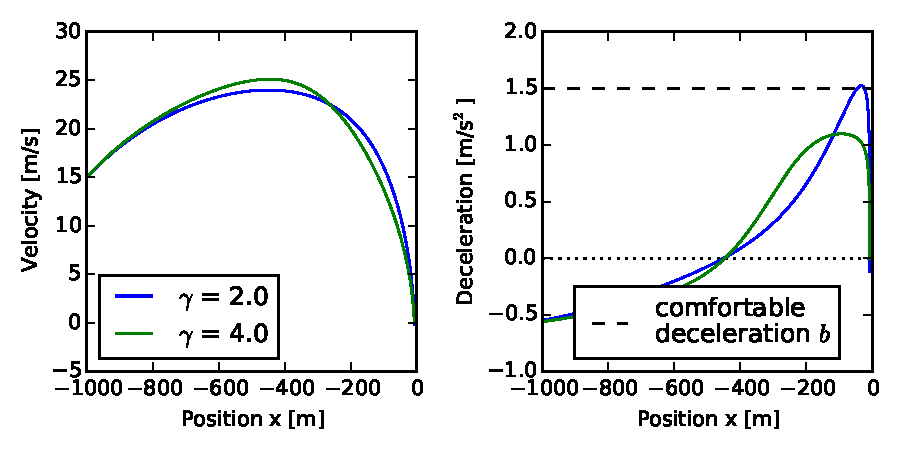
\includegraphics[width=5in]{../img/vel_profile.pdf}
    \caption{Velocity and deceleration profiles when approaching a stationary obstacle. The car starts at $x=\SI{-100}{m}$, while the obstacle is located at the origin. As expected, the deceleration for $\gamma=2$ tends towards $b$. For $\gamma=4$, the deceleration is \emph{initially} higher, but later the driver does not break as hard.}
    \label{fig:vel_profile}
\end{figure}

When simulating a single car approaching\footnote{The speed limit in this test was increased to $v_0 = \SI{30}{m/s}$.} a standing obstacle, we observe the acceleration behaviour represented in fig. \ref{fig:vel_profile}. During the accelerating phase (up to $x\approx\SI{-400}{m}$), there is little difference between $\gamma=2$ and $\gamma=4$. For $\gamma = 2$, the deceleration then tends towards $b$ as expected. The driver with $\gamma=4$ however breaks harder indeed, but only initially (up to $x\approx \SI{-100}{m}$). Later, having reduced the speed already more than required, the breaking is much softer than for $\gamma=2$ case.

The driver with $\gamma=4$ thus breaks earlier, avoiding having to break hard at the last moment. This explains why higher values for $\gamma$ enhance stability: the low-$\gamma$ driver rushes towards the obstacle, resulting in the number of cars involved in the perturbation growing quickly. The high-$\gamma$ drivers break early, avoiding to enter the perturbation themselves. Instead their behaviour signals the drivers further upstream the presence of an obstacle. This way, the perturbation can diffuse upstream.

